% Options for packages loaded elsewhere
\PassOptionsToPackage{unicode}{hyperref}
\PassOptionsToPackage{hyphens}{url}
%
\documentclass[
]{article}
\usepackage{amsmath,amssymb}
\usepackage{lmodern}
\usepackage{iftex}
\ifPDFTeX
  \usepackage[T1]{fontenc}
  \usepackage[utf8]{inputenc}
  \usepackage{textcomp} % provide euro and other symbols
\else % if luatex or xetex
  \usepackage{unicode-math}
  \defaultfontfeatures{Scale=MatchLowercase}
  \defaultfontfeatures[\rmfamily]{Ligatures=TeX,Scale=1}
\fi
% Use upquote if available, for straight quotes in verbatim environments
\IfFileExists{upquote.sty}{\usepackage{upquote}}{}
\IfFileExists{microtype.sty}{% use microtype if available
  \usepackage[]{microtype}
  \UseMicrotypeSet[protrusion]{basicmath} % disable protrusion for tt fonts
}{}
\makeatletter
\@ifundefined{KOMAClassName}{% if non-KOMA class
  \IfFileExists{parskip.sty}{%
    \usepackage{parskip}
  }{% else
    \setlength{\parindent}{0pt}
    \setlength{\parskip}{6pt plus 2pt minus 1pt}}
}{% if KOMA class
  \KOMAoptions{parskip=half}}
\makeatother
\usepackage{xcolor}
\usepackage[top=10mm, bottom=15mm, left=10mm, right=10mm]{geometry}
\usepackage{longtable,booktabs,array}
\usepackage{calc} % for calculating minipage widths
% Correct order of tables after \paragraph or \subparagraph
\usepackage{etoolbox}
\makeatletter
\patchcmd\longtable{\par}{\if@noskipsec\mbox{}\fi\par}{}{}
\makeatother
% Allow footnotes in longtable head/foot
\IfFileExists{footnotehyper.sty}{\usepackage{footnotehyper}}{\usepackage{footnote}}
\makesavenoteenv{longtable}
\usepackage{graphicx}
\makeatletter
\def\maxwidth{\ifdim\Gin@nat@width>\linewidth\linewidth\else\Gin@nat@width\fi}
\def\maxheight{\ifdim\Gin@nat@height>\textheight\textheight\else\Gin@nat@height\fi}
\makeatother
% Scale images if necessary, so that they will not overflow the page
% margins by default, and it is still possible to overwrite the defaults
% using explicit options in \includegraphics[width, height, ...]{}
\setkeys{Gin}{width=\maxwidth,height=\maxheight,keepaspectratio}
% Set default figure placement to htbp
\makeatletter
\def\fps@figure{htbp}
\makeatother
\setlength{\emergencystretch}{3em} % prevent overfull lines
\providecommand{\tightlist}{%
  \setlength{\itemsep}{0pt}\setlength{\parskip}{0pt}}
\setcounter{secnumdepth}{-\maxdimen} % remove section numbering
\usepackage{float} \floatplacement{figure}{H}
\ifLuaTeX
  \usepackage{selnolig}  % disable illegal ligatures
\fi
\IfFileExists{bookmark.sty}{\usepackage{bookmark}}{\usepackage{hyperref}}
\IfFileExists{xurl.sty}{\usepackage{xurl}}{} % add URL line breaks if available
\urlstyle{same} % disable monospaced font for URLs
\hypersetup{
  pdftitle={Figure outline / packet},
  hidelinks,
  pdfcreator={LaTeX via pandoc}}

\title{Figure outline / packet}
\usepackage{etoolbox}
\makeatletter
\providecommand{\subtitle}[1]{% add subtitle to \maketitle
  \apptocmd{\@title}{\par {\large #1 \par}}{}{}
}
\makeatother
\subtitle{Measuring the depth and breadth of Fkh1-FHA-dependent chromatin structure and replication function at replication origins}
\author{}
\date{\vspace{-2.5em}2022-11-07}

\begin{document}
\maketitle

\hypertarget{materials-and-methods}{%
\section{Materials and methods}\label{materials-and-methods}}

\hypertarget{sort-seq}{%
\subsection{SORT-seq}\label{sort-seq}}

\hypertarget{cutluring-and-sorting}{%
\subsubsection{Cutluring and sorting}\label{cutluring-and-sorting}}

Followed protocol as outlined in {[}@Batakou2020{]} with slight modifications. Briefly, 30 mL YPD cultures grown to 0.5 ODs/mL at 30°C. Harvested and fixed yeast in 70\% EtOH, storing overnight at 4°C.

\hypertarget{dna-extraction-library-prep-and-sequencing}{%
\subsubsection{DNA extraction, library prep, and sequencing}\label{dna-extraction-library-prep-and-sequencing}}

\hypertarget{data-processing-and-analysis}{%
\subsubsection{Data processing and analysis}\label{data-processing-and-analysis}}

\hypertarget{fkkh1-motif-mapping}{%
\subsection{FKKH1 motif mapping}\label{fkkh1-motif-mapping}}

\hypertarget{mnase-seq}{%
\subsection{MNase-seq}\label{mnase-seq}}

\hypertarget{benchwork}{%
\subsubsection{Benchwork}\label{benchwork}}

\hypertarget{dna-extraction-library-prep-and-sequencing-1}{%
\subsubsection{DNA extraction, library prep, and sequencing}\label{dna-extraction-library-prep-and-sequencing-1}}

\hypertarget{data-processing-and-analysis-1}{%
\subsubsection{Data processing and analysis}\label{data-processing-and-analysis-1}}

\hypertarget{results}{%
\section{Results}\label{results}}

\hypertarget{the-loss-of-functional-fkh1fha-impacts-replication-at-up-to-25-of-yeast-origins.}{%
\subsection{The loss of functional Fkh1FHA impacts replication at up to 25\% of yeast origins.}\label{the-loss-of-functional-fkh1fha-impacts-replication-at-up-to-25-of-yeast-origins.}}

\hypertarget{figure-1-establishing-the-big-q-and-our-sort-seq-experiment}{%
\subsubsection{Figure 1 (establishing the big Q and our SORT-seq experiment)}\label{figure-1-establishing-the-big-q-and-our-sort-seq-experiment}}

\textbf{Take-home:} \emph{Qualitatively and quantitatively, the loss of a functional Fkh1FHA changes replication dynamics at replication origins and perhaps even at termination events). Thus, more origins than the our original target PC cohort are affected by fkh1-R80A.}



\begin{figure}

{\centering 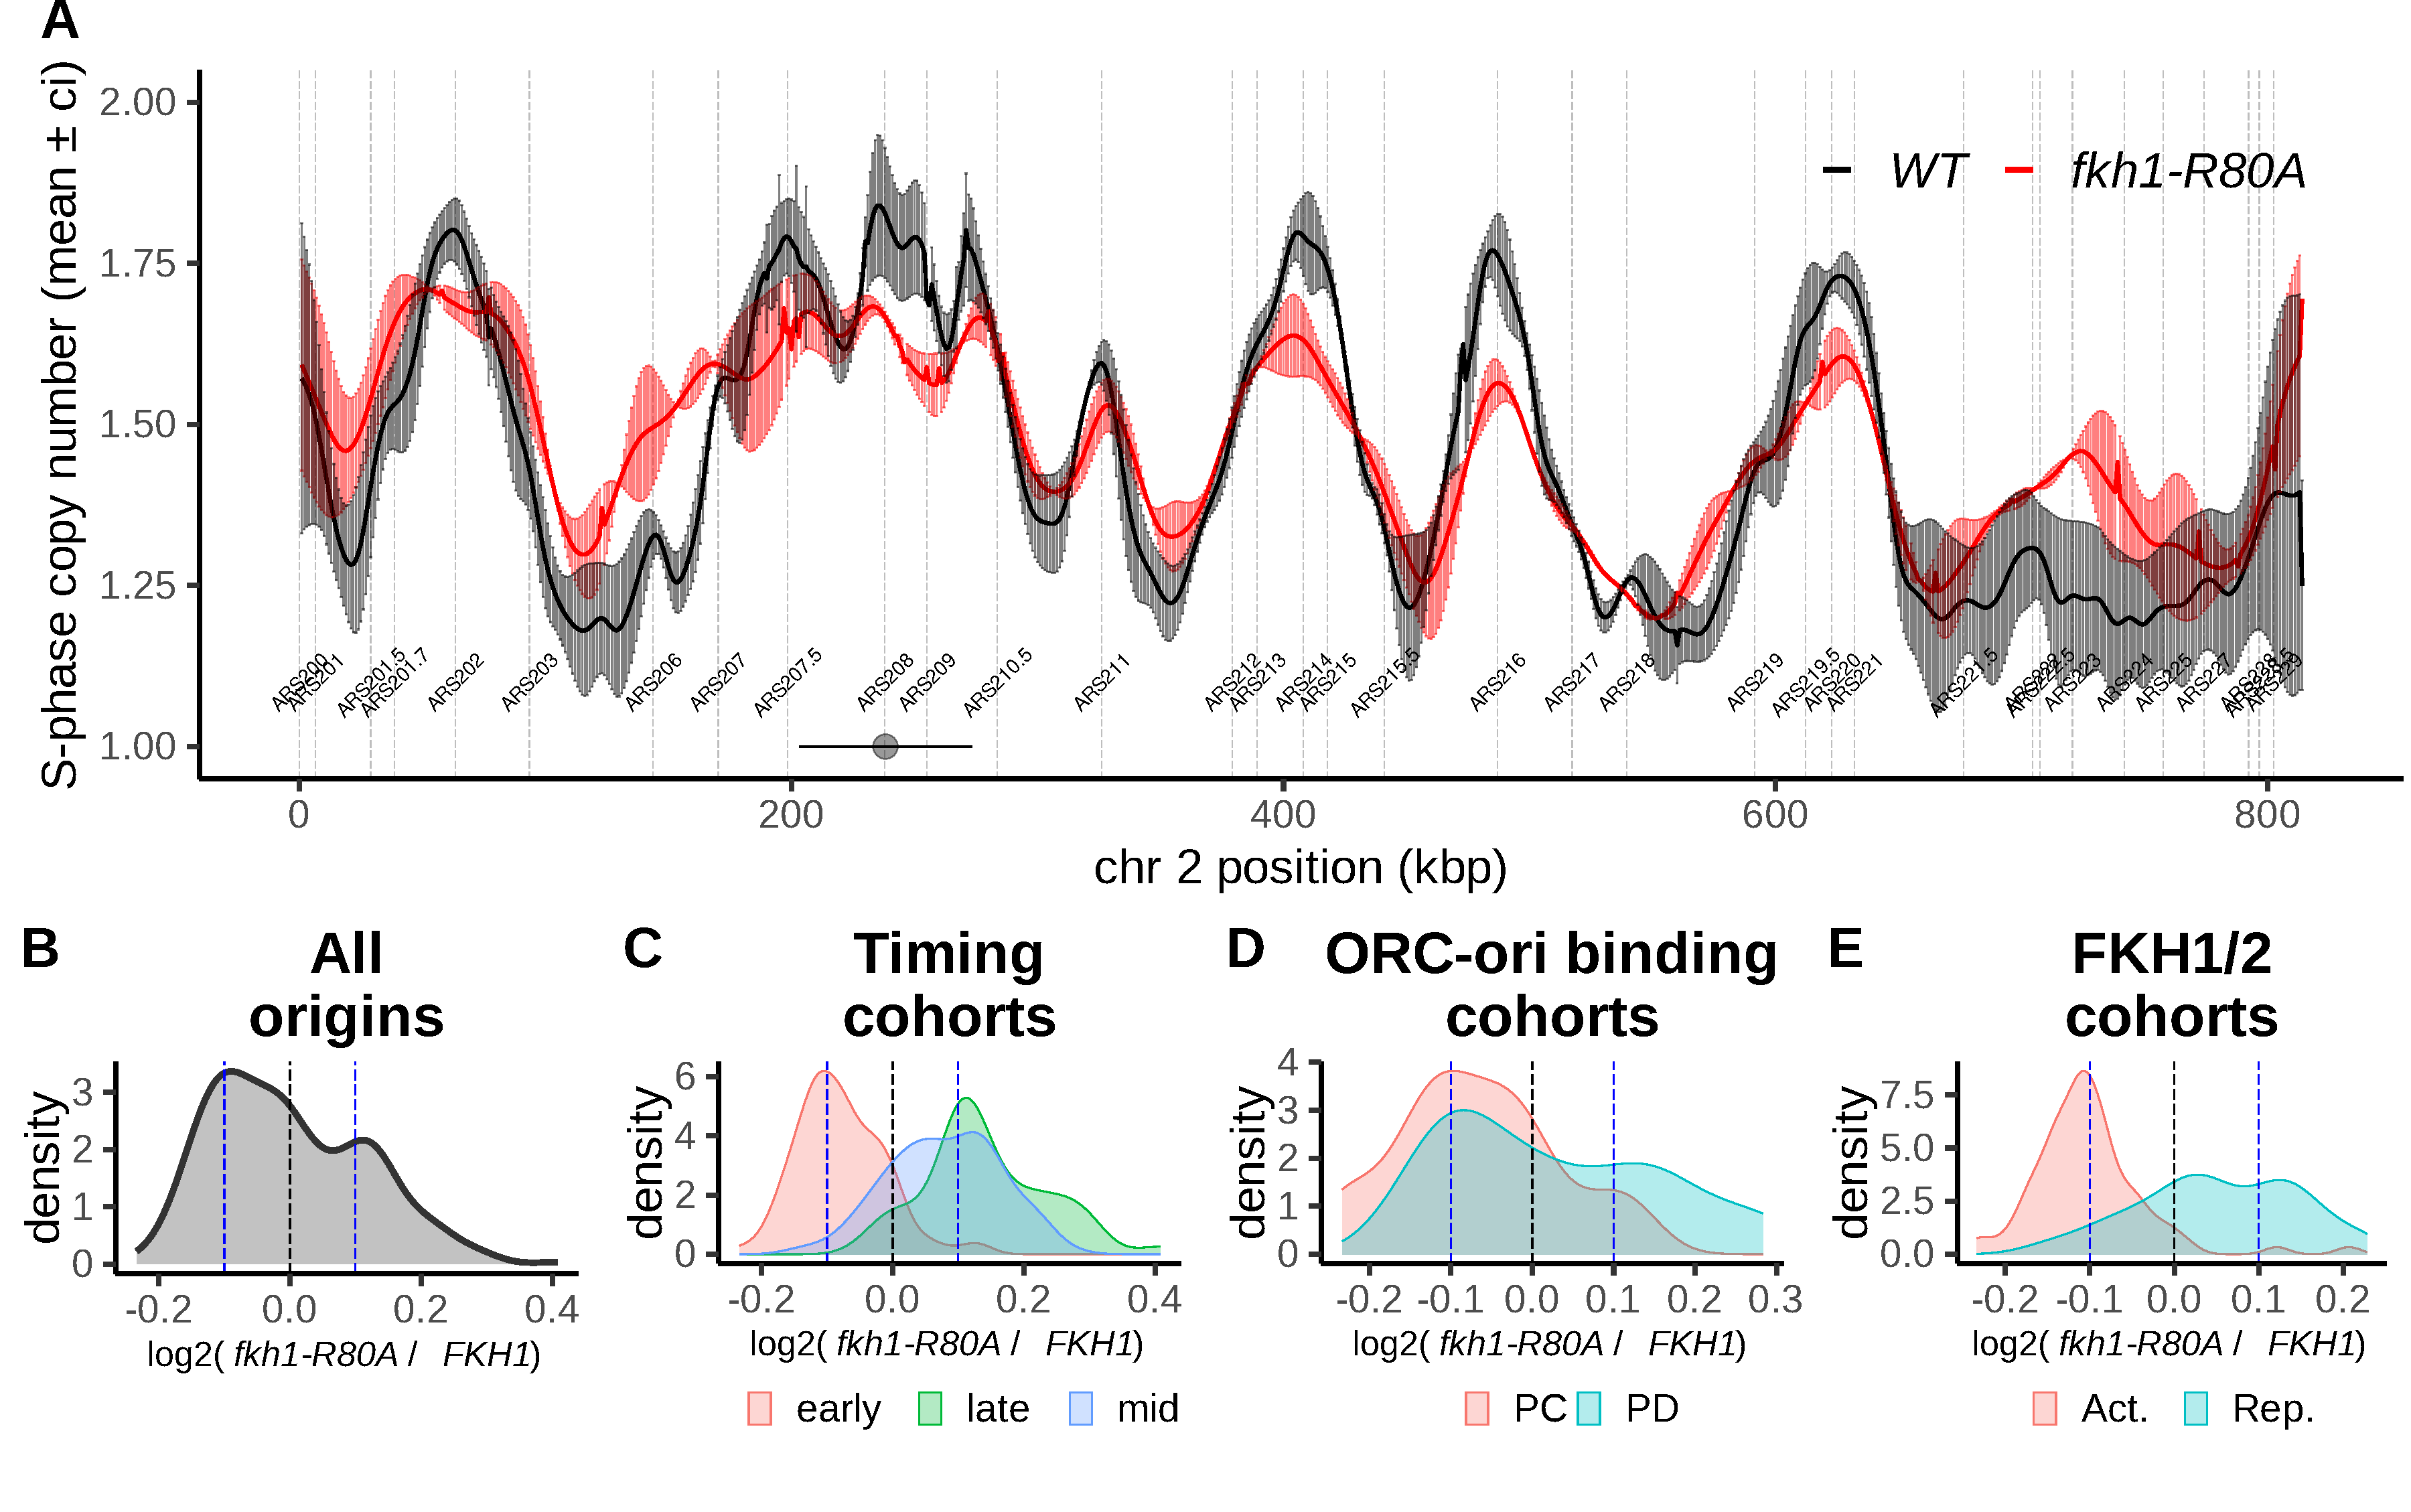
\includegraphics[width=0.85\linewidth]{./images/Figure_1_v_2022-11-08} 

}

\caption{\tiny Measuring replication in multiple \emph{FKH1} (3) and \emph{fkh1-R80A} (2) meiotic independents in unperturbed yeast cultures. \textbf{A.} S-phase copy numbers as means and 95\% confidence intervals measured across chromosome 2 in \emph{FKH1} (black) and \emph{fkh1-R80A} (red) cells. Sites of origins are labeled, with the position of the T-rich start of the ORC site indicated by vertical lines. The a 30 kbp window centered on the centromere is marked by a horizontal line with a central grey dot denoting the centromeric sequence. \textbf{B-E.} Smoothed density estimates of \emph{fkh1-R80A} / \emph{FKH1} S-phase copy number ratios for all confirmed origins (n = 392) and then selected cohorts defined by Trep (C - {[}@Yabuki2002{]}), ORC-origin binding cohorts (D - {[}@Hoggard2013{]}), and \emph{FKH1/2}-regulation (E - {[}@Knott2012{]}).}\label{fig:fig1}
\end{figure}

\hypertarget{supplemental-1-all-chromosomal-scans}{%
\subsubsection{Supplemental 1 (all chromosomal scans)}\label{supplemental-1-all-chromosomal-scans}}

\hypertarget{figure-2-cen-sequence-and-cen-origins-are-fha-sort-dependent-fkh1-r80a-sort-negative}{%
\subsection{\texorpdfstring{Figure 2 (CEN sequence and CEN origins are FHA-SORT-dependent / \emph{fkh1-R80A}-SORT-negative)}{Figure 2 (CEN sequence and CEN origins are FHA-SORT-dependent / fkh1-R80A-SORT-negative)}}\label{figure-2-cen-sequence-and-cen-origins-are-fha-sort-dependent-fkh1-r80a-sort-negative}}

\textbf{Take-home:} \emph{In contrast to a previous study that measured replication through BrdU-chip (Knott et al, 2012), our study suggests that normal replication through yeast centromeres is dependent on a functional Fkh1FHA.}

\begin{enumerate}
\def\labelenumi{\alph{enumi})}
\tightlist
\item
  Example scans~\\
\item
  Illustration of how CEN ratios were determined.~\\
\item
  Distribution of CEN ratios for all sixteen cens.~
\end{enumerate}

\hypertarget{supplemental-2-all-cen-scans}{%
\subsubsection{Supplemental 2 (all cen scans)}\label{supplemental-2-all-cen-scans}}

\hypertarget{figure-3-fkh1-match-frequency-by-sort-seq-cohorts}{%
\subsection{Figure 3 (FKH1 match frequency by SORT-seq cohorts)}\label{figure-3-fkh1-match-frequency-by-sort-seq-cohorts}}

\textbf{Take-home:} \emph{In contrast to the PC origins sensitive to fkh1-R80A in the NAR paper, fkh1-R80A-negative / FHA-SORT-dependent origins defined by the SORT-seq are characterized by a FKH1 match that overlaps the ORC binding site}

\hypertarget{figure-4-mnase-titration-reveals-global-change-in-accessibility-in-fkh1-r80a}{%
\subsection{\texorpdfstring{Figure 4 (MNase titration reveals global change in accessibility in \emph{fkh1-R80A})}{Figure 4 (MNase titration reveals global change in accessibility in fkh1-R80A)}}\label{figure-4-mnase-titration-reveals-global-change-in-accessibility-in-fkh1-r80a}}

\textbf{Data Tk} May save for reviewers or as a ``compromise'' for resubmission~

\textbf{Thought(s):} \emph{A figure to address the ``extent'' of chromatin accessibility governed by Fkh1-FHA. If no change between} FKH1* and \emph{fkh1-R80A}, then we will reserve for supplemental. We will start with asynchronous cells and then move to G1-arrested cells. If chromatin accessibility parallels the MNase-seq data, we may see opposing phenotypes between asynchronous and G1-arrested cells.*~

\hypertarget{figure-5-mnase-seq-experiment-validation}{%
\subsection{Figure 5 (MNase-seq experiment validation)}\label{figure-5-mnase-seq-experiment-validation}}

\textbf{Take-home:} \emph{We present data that suggest the Fkh1-FHA regulates chromatin structure as measured by MNase-seq experiments to such an extent that changes in MNase protection is evidenced for all confirmed origins and is G1-specific.}

\begin{enumerate}
\def\labelenumi{\alph{enumi})}
\tightlist
\item
  heats comparing confirmed to likely origins~\\
\item
  Quantification of heats~\\
\item
  Heats by region~\\
\item
  Quantification of heat regions.~
\end{enumerate}

\hypertarget{supplemental-3}{%
\subsubsection{Supplemental 3}\label{supplemental-3}}

Comparison of experimental replicates for the two genotypes\ldots{}

\hypertarget{figure-6-mnase-seq-experiment-with-cohorts-of-interest}{%
\subsection{Figure 6 (MNase-seq experiment with cohorts of interest)}\label{figure-6-mnase-seq-experiment-with-cohorts-of-interest}}

\textbf{Take-home:} \emph{As expected, Fkh1-FHA-dependent MNase protection is most evident in G1-phase and at FHA-sort-positive origins relative to FHA-sort-negative origins.}

As in figure 5, but with \emph{fkh1-R80A}-SORT-negative and \emph{fkh1-R80A}-SORT-positive.~

\hypertarget{supplemental-4}{%
\subsubsection{Supplemental 4}\label{supplemental-4}}

Comparison of experimental replicates for the two genotypes\ldots{}

\hypertarget{figure-7-mnase-seq-experiment-with-single-locus-plots-fkh1-matches}{%
\subsection{Figure 7 (MNase-seq experiment with single locus plots \& FKH1-matches)}\label{figure-7-mnase-seq-experiment-with-single-locus-plots-fkh1-matches}}

\textbf{Analysis Tk}

\end{document}
